\documentclass[11pt,a4paper]{article}

% These are extra packages that you might need for writing the equations:
\usepackage{amsmath}
\usepackage{amsfonts}
\usepackage{amssymb}
\usepackage{booktabs}
\usepackage{hyperref}
\usepackage{listings}
\usepackage{xcolor}
\lstset {language=C++,
		 basicstyle=\ttfamily,
         keywordstyle=\color{blue}\ttfamily,
         stringstyle=\color{red}\ttfamily,
         commentstyle=\color{purple}\ttfamily,
         morecomment=[l][\color{magenta}]{\#},
       	 basicstyle=\tiny}

% You need the following package in order to include figures in your report:
\usepackage{graphicx}

% With this package you can set the size of the margins manually:
\usepackage[left=2cm,right=2cm,top=2cm,bottom=2cm]{geometry}


\begin{document}

% Enter the exercise number, your name and date here:
\noindent\parbox{\linewidth}{
 \parbox{.25\linewidth}{ \large HPCSE I, Exercise 01 }\hfill
 \parbox{.5\linewidth}{\begin{center} \large Beat Hubmann \end{center}}\hfill
 \parbox{.2\linewidth}{\begin{flushright} \large Sep 30, 2018 \end{flushright}}
}
\noindent\rule{\linewidth}{2pt}

\section{Question 1}
Nothing to report.

\section{Question 2}
Nothing to report.

\section{Question 3}

\subsection{Task a)}
Assumptions for all subsequent calculations of operational intensity:
\begin{itemize}
\item{Cache is empty (i.e. cold)}
\item{"Memory transfer" implies transfer from random access memory (DRAM) to cache (typically L3 cache)}
\end{itemize}

\subsubsection{DAXPY}

\begin{equation}
y = \alpha x + y \quad \alpha \in \mathbb{R}; x, y \in \mathbb{R}^{n}
\end{equation}

According to table~\ref{tab:daxpy}, a DAXPY operation on $x, y \in \mathbb{R}^{n}$ requires $2n$ FLOPS and $3n$ memory accesses. By definition, \textbf{D}AXPY is a double precision operation and thus each involved element has a size of 8 bytes. The resulting total operational intensity is $I(n) = \frac{2n \: \text{FLOPS}}{3n \cdot 8 \: \text{bytes}} = \frac{1}{12} \: \text{ops/byte}$ and hence $\mathcal{O}(1)$.

\begin{table}[ht]
\centering
\begin{tabular}{@{\extracolsep{4pt}}lcccc}
\toprule
{}  & \multicolumn{2}{c}{FLOPS} & \multicolumn{2}{c}{memory accesses}\\
\cmidrule{2-3}
\cmidrule{4-5}
$i = 1,2, \ldots, n$ & multiply & add & read & write \\
\midrule
$n \: \text{times\ldots} $  & 1    & 1   & 2   & 1 \\
\bottomrule
\end{tabular}
\caption{DAXPY operations per element $i \in \{1, 2, \ldots, n\}$}\label{tab:daxpy}
\end{table}

\subsubsection{SGEMV}

\begin{equation}
y = Ax + y \quad x, y \in \mathbb{R}^{n}; A \in \mathbb{R}^{n \times n}
\end{equation}

According to table~\ref{tab:sgemv}, a SGEMV operation on $x, y \in \mathbb{R}^{n}$ requires $2n^2 + n$ FLOPS and $2n^2 + 2n$ memory accesses. To make things easier we focus on the asymptotic bound and only consider the second-order terms. By definition, \textbf{S}GEMV is a single precision operation and thus each involved element has a size of 4 bytes. The resulting total asymptotic operational intensity is $I(n) = \frac{2n^2\: \text{FLOPS}}{2n^2\cdot 4 \: \text{bytes}} = \frac{1}{4} \: \text{ops/byte}$ and hence $\mathcal{O}(1)$.

\begin{table}[ht]
\centering
\begin{tabular}{@{\extracolsep{4pt}}lcccc}
\toprule
{}  & \multicolumn{2}{c}{FLOPS} & \multicolumn{2}{c}{memory accesses}\\
\cmidrule{2-3}
\cmidrule{4-5}
$i = 1,2, \ldots, n$ & multiply & add   & read   & write \\
\midrule
$n \: \text{times\ldots} $                    & $n$      & $n+1$ & $2n+1$ & 1 \\
\bottomrule
\end{tabular}
\caption{SGEMV operations per element $i \in \{1, 2, \ldots, n\}$}\label{tab:sgemv}
\end{table}


\subsubsection{DGEMM}

\begin{equation}
C = AB + C \quad A,B,C \in \mathbb{R}^{n \times n}
\end{equation}

Based on the hint given in the task description, we assume that $n$ and thus the matrices $A, B, C$ are small enough to fit in the cache concurrently and do not require multiple reads during a single DGEMM operation. According to table~\ref{tab:dgemm}, a DGEMM operation on $B, C \in \mathbb{R}^{n \times n}$ requires $2n^3 + n^2$ FLOPS and only $4n^2$ memory accesses because of the above assumption about $n$ versus cache size. As for SGMEV above, we focus on the higher order terms for the following calculations. By definition, \textbf{D}GEMM is a double precision operation and thus each involved element has a size of 8 bytes. The resulting total asymptotic operational intensity is $I(n) = \frac{2n^3\: \text{FLOPS}}{4n^2\cdot 8 \: \text{bytes}} = \frac{n}{16} \: \text{ops/byte}$ and hence $\mathcal{O}(n)$.

\begin{table}[ht]
\centering
\begin{tabular}{@{\extracolsep{4pt}}lcccc}
\toprule
{}  & \multicolumn{2}{c}{FLOPS} & \multicolumn{2}{c}{memory accesses}\\
\cmidrule{2-3}
\cmidrule{4-5}
$i,j = 1,2, \ldots, n$ & multiply & add   & read   & write \\
\midrule
$n\cdot n \: \text{times\ldots} $                    & $n$      & $n+1$ & $3$ & 1 \\
\bottomrule
\end{tabular}
\caption{DGEMM operations per element $i, j \in \{1, 2, \ldots, n\}$}\label{tab:dgemm}
\end{table}


\subsection{Task b)}

\begin{equation}
u_{i}^{n+1} = u_{i}^{n} + \frac{\Delta t \alpha}{\Delta x^2}(u_{i-1}^{n} - 2u_{i}^{n} + u_{i+1}^{n})
\label{eqn:1d_diffusion}
\end{equation}

Based on equation~(\ref{eqn:1d_diffusion}) and considering that $\frac{\Delta t \alpha}{\Delta x^2}$ is a fixed value which can be precalculated and stored, there are 3 additions and 2 multiplications for a total of 5 FLOPS per grid point. As for DGEMM in the previous task, we now must make assumptions about the problem size versus the cache size (the cache size being a potential bottleneck): It would be most realistic but also most cumbersome for our calculations to assume that some part of the problem fits in a cache of limited but realistic size and that we have to deal with a mix of compulsory and capacity cache misses. At the extreme ends of the cache size-vs-problem size scale we could take up either the assumption of an infinite cache and thus only one read and one write operation per grid point or the assumption of zero cache with a worst case maximum of four reads and one write per grid point. Assuming we are dealing with double precision data (8 bytes per element), we can thus make the following estimations: $I(N)_{\text{max}} = \frac{5\: \text{FLOPS}}{2\cdot8 \: \text{bytes}}=\frac{5}{16}\: \text{ops/byte}$ and $I(N)_{\text{min}} = \frac{5\: \text{FLOPS}}{5\cdot8 \: \text{bytes}}=\frac{1}{8}\: \text{ops/byte}$ with the realistic asymptotic operational intensity bounded as in equation~(\ref{eqn:task3b}).
\begin{equation}
0.125  \: \text{ops/byte} \leq I(N) \leq 0.3125  \: \text{ops/byte}
\label{eqn:task3b}
\end{equation}

\section{Question 4}

\subsection{Task a)}
Based on the link~\cite{intel} given in the task description, the CPU used is of the Haswell generation, has 12 cores with a processor base frequency of 2.50 GHz and can use the AVX2 instruction set. As nicely summarized in~\cite{nasa}, AVX2 introduced 256-bit (i.e. 4 times 64-bit double-precision elements) floating-point fused multiply-add (FMA) support which allows for 16 double precision floating point operations per cycle (2 FMA execution units each able to execute 2 operations per cycle). In total, this gives $\pi = 12 \times 2.5 \times 10^9 \frac{\text{cycle}}{s} \times 16 \frac{\text{FLOPS}}{\text{cycle}} = 480 \frac{\text{GFLOPS}}{s}$.\\
 According to~\cite{intel}, the fastest memory supported by the CPU is DDR4 memory running at 2133 MHz on four memory channels of size 64 bit each (the 256 bit as described above divided by 4). We thus get a maximum memory bandwidth of $\beta = 2133 \times 10^6 \frac{\text{cycle}}{s} \times 256 \frac{\text{bit}}{\text{cycle}} = 546.048 \frac{\text{Gbit}}{s} = 68.256 \frac{\text{Gbyte}}{s}$ which conveniently also is equal to the \textit{Max Memory Bandwith} of 68GB/s indicated on~\cite{intel} itself.  


\subsection{Task b)}
\subsubsection{$I_b$ when in operating in balance}
As described in~\cite{kou}, the ridge point is where both the CPU and the memory bandwidth are fully exploited and is situated at the intersection of $\pi$ and $I \times \beta$ in a log-log plot of operational intensity $I$ vs $\text{GFLOPS}/s$.\\
In specific, for a full node of Euler II we have $I_b = \frac{\pi}{\beta} = \frac{960 \frac{\text{GFLOPS}}{s}}{136.6\frac{\text{Gbyte}}{s}} \approx 7 \: \text{ops/byte}$.

\subsubsection{$P_{\text{peak}}$}
Also as per the source and calculations cited above, we have that $P_{\text{peak}}(I) = \text{min}(\pi, I\times \beta)$ where $\pi, \beta$ are fixed hardware properties as described above.

\subsubsection{memory bound vs compute bound}
A code is memory bound if its operational intensity $I$ is smaller than the calculated balanced operational intensity $I_b$: $I < I_b$. Likewise, a code is compute bound if we have that $I > I_b$.
The possible optimisations differ according to the bound: For memory bound code, it is recommended~\cite{kou} to first minimise conflict caches misses by data reordering and then to minimise capacity cache misses by reordering and non-temporal writes. All this is to increase operational intensity $I$.\\
For compute bound codes, it is harder to find optimisations as there is no point in further increasing operational intensity. Possible measures include use of SSE/AVX instructions and/or reductions in precision.

\subsection{Task c)}
According to~\cite{euler}, a full compute node of Euler II has two sockets each according to the above Xeon E5-2680v3 CPU and memory bandwidth specifications $\pi, \beta$ with a total of 24 cores per node. Based on the computations This makes for a roofline diagram as in figure~\ref{fig:roofline}.

\begin{figure}[ht]
\begin{center}
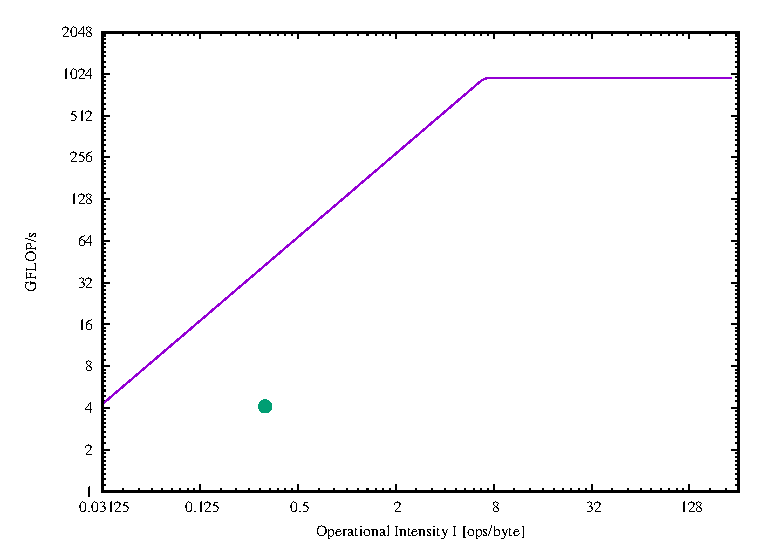
\includegraphics[scale=0.9]{roofline.eps} 
\end{center}
\caption{Roofline diagram for full compute node of Euler II; measured value of task d).}
\label{fig:roofline}
\end{figure}

\subsection{Task d)}
Based on the code with an attempted CPU data cache flush given in appendix~\ref{app} compiled with GCC 4.8.2 using the flags \lstinline{-fopenmp} \lstinline{-std=c++11} \lstinline{-O3} \lstinline{-march=native} \lstinline{-funroll-loops} (using OpenMP only to get a simple way to measure time), repeated measurements on Euler II result in a performance of about $4.1 \frac{\text{GFLOPS}}{s}$ short of the theoretically achievable single thread/single channel maximum of $5 \frac{\text{GFLOPS}}{s}$. This position is marked by a green dot in figure~\ref{fig:roofline}. We therefore conclude that the chosen implementation falls into to the memory bound region as described above. Potential reasons for not fully utilising the hardware are the naive implementation (unbalanced adds/multiplies) as well as only using a single thread. A first measure would be to use OpenMP to use all available threads on the CPU's cores.

\begin{thebibliography}{99}

\bibitem{nasa}
	NASA,
 	\emph{Haswell Processors},
	online (\url{https://www.nas.nasa.gov/hecc/support/kb/haswell-processors_492.html}),
 	accessed 30-Sep-2018.
 
\bibitem{intel}
	Intel Corporation,
	\emph{Intel Xeon Processor E5-2680 v3 Product Specifications},
	online (\url{https://ark.intel.com/products/81908/}),
	accessed 30-Sep-2018.
	
\bibitem{euler}
	ETH Zurich,
 	\emph{scientific computing wiki: Euler},
	online (\url{https://scicomp.ethz.ch/wiki/Euler#Euler_II}),
 	accessed 30-Sep-2018.	

\bibitem{kou}
	Petros Koumoutsakos,
	\emph{HPCSE I Lecture Notes},
	online (\url{http://www.cse-lab.ethz.ch/wp-content/uploads/2018/09/HPCSE_I_1_Intro.pdf}),
	accessed 30-Sep-2018.

\end{thebibliography}


\appendix
\section{Question 4, task d)}\label{app}
\lstinputlisting{ex01_q4_task_d.cpp}
\end{document}